% This is part of Un soupçon de mathématique sans être agressif pour autant
% Copyright (c) 2012
%   Laurent Claessens
% See the file fdl-1.3.txt for copying conditions.

\chapter{Statistiques descriptives}

%+++++++++++++++++++++++++++++++++++++++++++++++++++++++++++++++++++++++++++++++++++++++++++++++++++++++++++++++++++++++++++
\section{Regardons des graphiques}
%+++++++++++++++++++++++++++++++++++++++++++++++++++++++++++++++++++++++++++++++++++++++++++++++++++++++++++++++++++++++++++

%---------------------------------------------------------------------------------------------------------------------------
\subsection{Émissions par secteurs}
%---------------------------------------------------------------------------------------------------------------------------

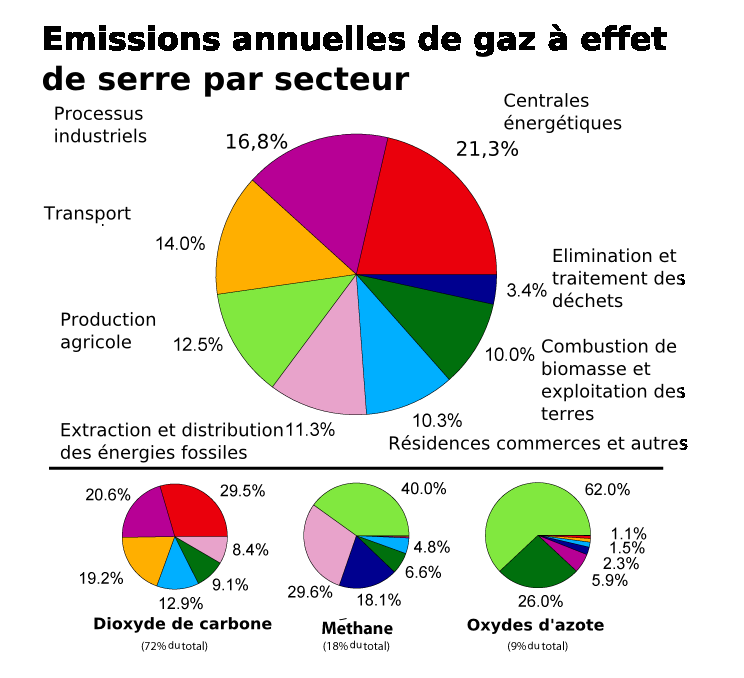
\includegraphics[width=17cm]{Emission_de_GES.png}

\begin{enumerate}
    \item
        Quel est le secteur qui émets le plus ?
    \item
        Est-ce que l'agriculture émet beaucoup de dioxyde de carbone ?
    \item
        À partir des deux graphiques du bas, est-ce que vous êtes capables de retrouver le \( 12.5\%\) de l'agriculture donnés dans le graphique du haut ?
\end{enumerate}

%---------------------------------------------------------------------------------------------------------------------------
\subsection{Découvertes de pétrole}
%---------------------------------------------------------------------------------------------------------------------------

Regardons un instant le graphique suivant.

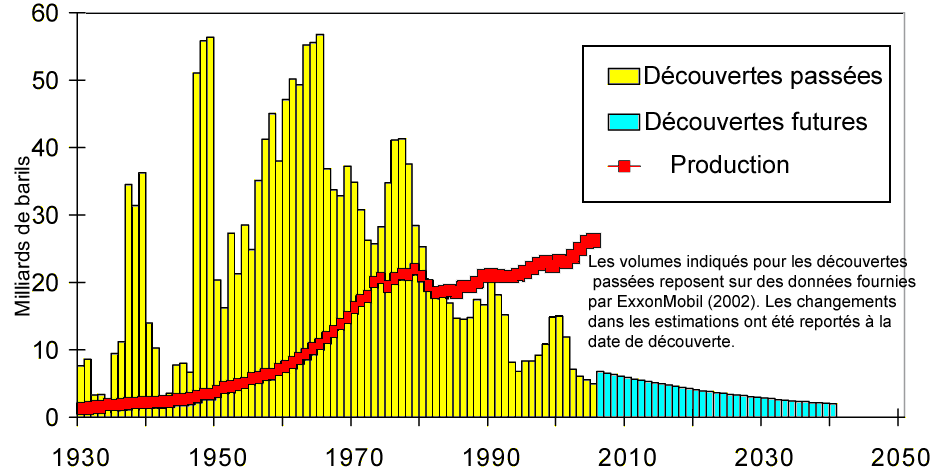
\includegraphics[width=17cm]{Decouvertes-petrole.png}

\begin{enumerate}
    \item
        Quelle est l'année où on a découvert le plus de pétrole ?
    \item
        Quelle est l'année où on a consommé le plus de pétrole ?
    \item
        En quelles années on a consommé autant qu'on a découvert ?
    \item
        Que pensez-vous de l'affirmation «ce qui reste comme réserve est la surface jaune au-dessus de la ligne rouge» ?
\end{enumerate}

%---------------------------------------------------------------------------------------------------------------------------
\subsection{Températures}
%---------------------------------------------------------------------------------------------------------------------------

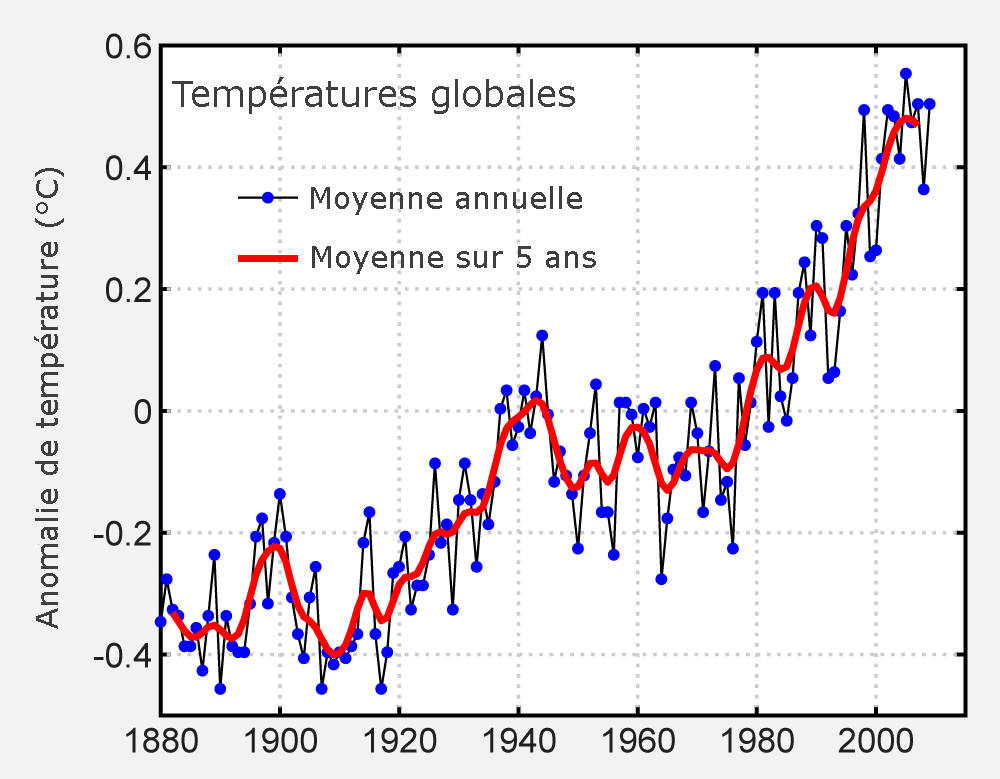
\includegraphics[width=17cm]{Instrumental_Temperature_Record_fr.png}

Le zéro de ce graphique est la moyenne 1961-1990.

\begin{enumerate}
    \item
        Quelle est la dernière année «normale» ?
    \item
        Quelle est l'année la plus chaude ?
    \item
        Quelle est l'année la plus froide ?
\end{enumerate}

Lire le tableau suivant :
\begin{center}
\begin{tabular}[h]{|c|c|c|c|c|c|c|c|c|}
année&
2001&
2002&
2003&
2004&
2005&
2006&
2007&
2008\\
consommation (Mb/j)&
76,8&
77,7&
79,1&
81,8&
83,1&
83,8&
84,9&
84,5
\end{tabular}
\end{center}

Calculer le pourcentage d'augmentation année par année. Que s'est-il passé en 2008 ?


\chapter{À faire fonctionner}

Les graphiques montrent
\begin{enumerate}
    \item

        À la figure \ref{LabelFigautomaticDSpcb}, \( y=\) proportion des étudiants ayant obtenu plus que \( x\)
    \item
        À la figure \ref{LabelFigautomaticDSpbt}, \( y=\) moyenne des étudiants ayant obtenu plus que \( x\). Par construction, le tout premier point de ce graphique est la moyenne de tout le groupe.
    \item
        À la figure \ref{LabelFigautomaticDSavb}, \( y=\) proportion des étudiants ayant obtenu dans \( \mathopen[ x-0.5 , x+0.5 \mathclose]\).
\end{enumerate}

\newcommand{\CaptionFigautomaticDSpcb}{Moyenne des étudiants ayant obtenus plus que \( x\)}
\input{Fig_automaticDSpcb.pstricks}

\newcommand{\CaptionFigautomaticDSpbt}{Proportion des étudiants ayant obtenus plus que \( x\)}
\input{Fig_automaticDSpbt.pstricks}

\newcommand{\CaptionFigautomaticDSavb}{proportion des étudiants ayant obtenu dans \( x\pm 0.5\)}
\input{Fig_automaticDSavb.pstricks}

\chapter{Exercices}

%+++++++++++++++++++++++++++++++++++++++++++++++++++++++++++++++++++++++++++++++++++++++++++++++++++++++++++++++++++++++++++
\section{Repères, distances, milieu}
%+++++++++++++++++++++++++++++++++++++++++++++++++++++++++++++++++++++++++++++++++++++++++++++++++++++++++++++++++++++++++++

\Exo{Seconde-0001}
\Exo{Seconde-0002}
\Exo{Seconde-0003}
\Exo{Seconde-0004}
\Exo{Seconde-0005}
\Exo{Seconde-0006}
\Exo{Seconde-0007}
\Exo{Seconde-0008}
\Exo{Seconde-0009}
\Exo{Seconde-0010}
\Exo{Seconde-0011}
\Exo{Seconde-0012}
\Exo{Seconde-0013}

%+++++++++++++++++++++++++++++++++++++++++++++++++++++++++++++++++++++++++++++++++++++++++++++++++++++++++++++++++++++++++++
\section{Petits exercices de calcul mental}
%+++++++++++++++++++++++++++++++++++++++++++++++++++++++++++++++++++++++++++++++++++++++++++++++++++++++++++++++++++++++++++

\Exo{Seconde-0014}
\Exo{Seconde-0015}
\Exo{Seconde-0016}
\Exo{Seconde-0017}
\Exo{Seconde-0018}
\Exo{Seconde-0019}
\Exo{Seconde-0020}
\Exo{Seconde-0021}
\Exo{Seconde-0022}
\Exo{Seconde-0023}
\Exo{Seconde-0024}
\Exo{Seconde-0025}
\Exo{Seconde-0026}
\Exo{Seconde-0027}
\Exo{Seconde-0028}
\Exo{Seconde-0029}
\Exo{Seconde-0030}
\Exo{Seconde-0031}
\Exo{Seconde-0032}
\Exo{Seconde-0033}
\Exo{Seconde-0034}
\Exo{Seconde-0035}
\Exo{Seconde-0036}
\Exo{Seconde-0037}
\Exo{Seconde-0038}
\Exo{Seconde-0039}
\Exo{Seconde-0040}
\Exo{Seconde-0041}
\Exo{Seconde-0042}
\Exo{Seconde-0043}
\Exo{Seconde-0044}
\Exo{Seconde-0045}
\Exo{Seconde-0046}
\Exo{Seconde-0047}
\Exo{Seconde-0048}
\Exo{Seconde-0049}
\Exo{Seconde-0050}
\Exo{Seconde-0051}
\Exo{Seconde-0052}
\Exo{Seconde-0053}
\Exo{Seconde-0054}
\Exo{Seconde-0055}
\Exo{Seconde-0056}
\Exo{Seconde-0057}
\Exo{Seconde-0058}
\Exo{Seconde-0059}
\Exo{Seconde-0060}
\Exo{Seconde-0061}
\Exo{Seconde-0062}
\Exo{Seconde-0063}
\Exo{Seconde-0064}
\Exo{Seconde-0065}
\Exo{Seconde-0066}
\Exo{Seconde-0067}
\Exo{Seconde-0068}
\Exo{Seconde-0069}
\Exo{Seconde-0070}
\Exo{Seconde-0071}
\Exo{Seconde-0072}
\Exo{Seconde-0073}
\Exo{Seconde-0074}
\Exo{Seconde-0075}
\Exo{Seconde-0076}
\Exo{Seconde-0077}
\Exo{Seconde-0078}
\Exo{Seconde-0079}
\Exo{Seconde-0080}
\Exo{Seconde-0081}
\Exo{Seconde-0082}
\Exo{Seconde-0083}
\Exo{Seconde-0084}
\Exo{Seconde-0085}
\Exo{Seconde-0086}
\Exo{Seconde-0087}
\Exo{Seconde-0088}
\Exo{Seconde-0089}
\Exo{Seconde-0090}
\Exo{Seconde-0091}
\Exo{Seconde-0092}
\Exo{Seconde-0093}
\Exo{Seconde-0094}
\Exo{Seconde-0095}
\Exo{Seconde-0096}
\Exo{Seconde-0097}
\Exo{Seconde-0098}
\Exo{Seconde-0099}
\Exo{Seconde-0100}
%+++++++++++++++++++++++++++++++++++++++++++++++++++++++++++++++++++++++++++++++++++++++++++++++++++++++++++++++++++++++++++

